\section{Descrição do Sistema}
\begin{quote}
    O quadricóptero, ou quadrirrotor, é um tipo de helicóptero com quatro rotores. Os rotores ficam 
    voltados para cima e são posicionados em forma de quadrado, todos à mesma distância do centro de 
    massa do equipamento. O controle é realizado por meio do ajuste da velocidade angular dos rotores, 
    que são acionados por motores elétricos. — LUUKKONEN, 2011 \cite{luukkonen} (adaptado)
\end{quote}

A Figura \ref{fig:modelo} abaixo ilustra o modelo do quadcóptero considerado nesse trabalho, incluindo 
as velocidades angulares $\omega$, os torques $\tau$ e as forças $f$ de cada um dos rotores. Além disso, 
representa os dois sistemas de coordenadas necessários para a modelagem: o ``Body Frame'', relativo ao 
sistema de coordenadas móvel que tem o centro do drone como encontro dos eixos e no qual medimos as angulações 
do aparelho, e o ``Inertial Frame'', relativo ao sistema de coordenadas fixo no solo que é utilizado para 
obtenção das coordenadas de posição no espaço.

\begin{figure}[h!]
    \centering
    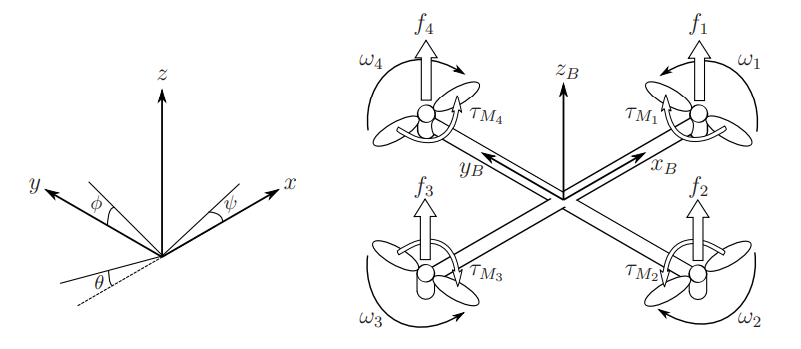
\includegraphics[width=0.8\textwidth]{figs/desenho_drone.png}
    \caption{Esquema de um quadcóptero. \cite{luukkonen}}
    \label{fig:modelo}
\end{figure}

\subsection{Dinâmica}

Passando para uma interpretação mais matemática do modelo do drone, é importante explicitar as equações diferenciais 
que regem a dinâmica do sistema, porém, antes disso, é preciso definir suas variáveis de estado (ver Tabela \ref{tab:vars}) 
e seus parâmetros (ver Tabela \ref{tab:params}).

\begin{table}[h!]
    \centering
    \caption{Variáveis de estado do sistema}
    \begin{tabular}{|c|c|c|}
        \hline
        \emph{Variáveis} & \emph{Descrição} & \emph{Unidade} \\ \hline
        ${x, y, z}$& Posição do drone nos eixos x, y e z & m \\ \hline
        ${\phi, \theta, \psi}$& Ângulo de rotação em torno dos eixos x, y e z & rad \\ \hline
        ${u, v, w}$& Velocidade do drone nos eixos x, y e z & m/s \\ \hline
        ${p, q, r}$& Velocidade angular da rotação em torno dos eixos x, y e z & rad/s \\ \hline
    \end{tabular}
    \label{tab:vars}
\end{table}

\vspace{-1cm}

\begin{center}
    \begin{longtable}{|c|c|c|c|} % <-- note o uso de p{largura}
        \caption{Parâmetros do sistema} \vspace{-0.7cm}
        \label{tab:params}
        \hline
        \emph{Parâmetros} & \emph{Descrição} & \emph{Valores} & \emph{Unidade} \\
        \hline
        \endfirsthead
        \endhead

        $\mathtt{m}$ & Massa do drone & $0,468$ &kg \\ \hline
        $\mathtt{g}$ & Aceleração da gravidade & $9,81$ & m/s² \\ \hline
        $\mathtt{I_{xx}}$ & Momento de inércia em torno do eixo x & $4,856 \cdot 10^{-3}$ & kg·m² \\ \hline
        $\mathtt{I_{yy}}$ & Momento de inércia em torno do eixo y & $4,856 \cdot 10^{-3}$ & kg·m² \\ \hline
        $\mathtt{I_{zz}}$ & Momento de inércia em torno do eixo z & $8,801 \cdot 10^{-3}$ & kg·m² \\ \hline
        $\mathtt{A_{xx}}$ & Arrasto em torno do eixo x & $0,25$ & kg·m²/s \\ \hline
        $\mathtt{A_{yy}}$ & Arrasto em torno do eixo y & $0,25$ & kg·m²/s \\ \hline
        $\mathtt{A_{zz}}$ & Arrasto em torno do eixo z & $0,25$ & kg·m²/s \\ \hline
        $\mathtt{l}$ & Distância do centro de massa até os rotores & $0,225$ & m \\ \hline
        $\mathtt{b}$ & Constante de empuxo dos rotores & $1,14 \cdot 10^{-7}$ & N$\cdot s^{2}$/$rad^{2}$ \\ \hline
        $\mathtt{k}$ & Constante de torque dos rotores & $2,98 \cdot 10^{-6}$ & N$\cdot s^{2}$/$rad^{2}$ \\ \hline
        $\mathtt{u_1, u_2, u_3, u_4}$ & Velocidade angular do rotor 1, 2, 3 e 4 & X & rad/s \\ \hline
    \end{longtable}
\end{center}

\vspace{-1.5cm}

Com isto definido, a seguir estão as doze equações diferenciais que descrevem o comportamento dinâmico do drone:

\vspace{+0.5cm}

\begin{minipage}{0.5\textwidth}
    \begin{equation*}
        \begin{aligned}
            &\dot{{x}} = {w}({s_{\phi}s_{\psi}} + {c_{\phi}c_{\psi}c_{\theta}}) - {v}({c_{\phi}c_{\psi}} - {c_{\phi}c_{\psi}c_{\theta}}) \\
            &\hspace{1.5cm} + {uc_{\psi}c_{\theta}}\\
            &\dot{{y}} = {v}({c_{\phi}c_{\psi}} + {s_{\phi}s_{\psi}s_{\theta}}) - {w}({c_{\psi}s_{\phi}} - {c_{\phi}s_{\psi}s_{\theta}}) \\
            &\hspace{1.5cm} + {uc_{\theta}s_{\psi}}\\
            &\dot{{z}} = {wc_{\phi}c_{\theta}} - {us_{\theta}} + {vc_{\theta}s_{\phi}}\\
            &\dot{{\phi}} = {p} + {qs_{\phi}t_{\theta}} + {rs_{\phi}t_{\theta}}\\
            &\dot{{\theta}} = {qc_{\phi}} - {rs_{\phi}}\\
            &\dot{{\psi}} = {r\left(\frac{c_{\phi}}{c_{\theta}}\right)} + {q\left(\frac{s_{\phi}}{c_{\theta}}\right)}
        \end{aligned}
    \end{equation*}
\end{minipage}
\hfill
\begin{minipage}{0.45\textwidth}
    \begin{equation*}
        \begin{aligned}
            &\dot{{u}} = {rv} - {qw} + {gs_{\theta}} - \frac{{A_{xx}}{u}}{{m}}\\
            &\dot{{v}} = {pw} - {ru} - {gc_{\theta}s_{\phi}} - \frac{{A_{yy}}{v}}{{m}}\\
            &\dot{{w}} = {qu} - {pv} + {gc_{\phi}c_{\theta}} + {\frac{T}{m}} - \frac{{A_{zz}}{w}}{{m}}\\
            &\dot{{p}} = {\frac{1}{I_{xx}}\left[{\tau_x + (I_{yy} - I_{zz})qr}\right]}\\
            &\dot{{q}} = {\frac{1}{I_{yy}}\left[{\tau_y + (I_{zz} - I_{xx})pr}\right]}\\
            &\dot{{r}} = {\frac{1}{I_{zz}}\left[{\tau_z + (I_{xx} - I_{yy})pq}\right]}
        \end{aligned}
    \end{equation*}
\end{minipage}

\vspace{+0.5cm}

Onde $s_{\gamma}$ e $c_{\gamma}$ são as funções seno e cosseno, respectivamente, de um ângulo $\gamma$.

\subsection{Ações de Controle}

\begin{figure}[h!]
    \centering
    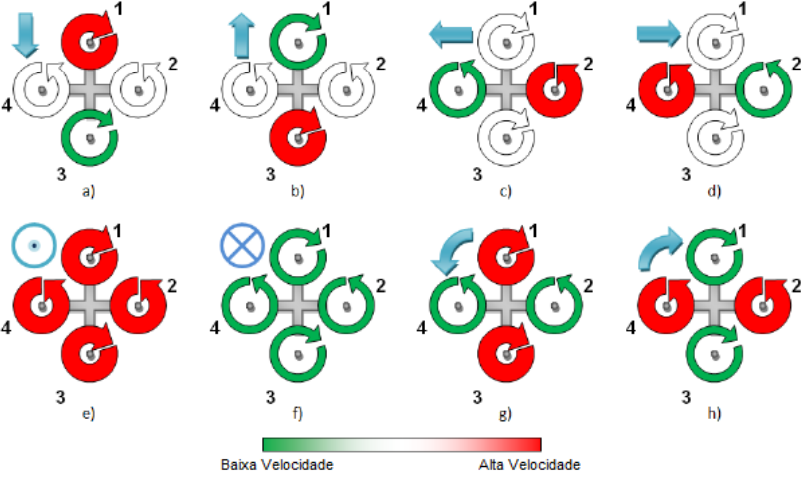
\includegraphics[width=0.65\textwidth]{figs/mov_drone.png}
    \caption{Correspondências entre velocidades angulares e movimentações do crone. \cite{usp}}
    \label{fig:movimento}
\end{figure}

\pagebreak

Por fim, a Figura \ref{fig:movimento} acima detalha todas as relações entre as potências das velocidades angulares 
dos rotores com cada um dos movimentos que o drone é capaz de fazer.
Como é possível notar, todos os movimentos precisam da ação conjunta dos rotores para ser realizado, de modo que 
as ações do controlador, as quais buscam controlar as saídas do modelo (como, por exemplo, movimentação em $z$ ou 
angulação em $\phi$), são dadas em funções dessas saídas, o que torna necessária uma conversão entre as ações dadas 
pelo controlador e aquelas que serão efetivamente enviadas para os motores. Foi por esse motivo que se decidiu criar 
um ``bloco'' a mais no diagrama de controle que fosse responsável apenas por fazer essa conversão. Assim, as relações 
que são usadas para tal são as seguintes:
\begin{eqnarray}
    U_1 &=& U_z - U_\theta - U_\psi + \text{bias} \\
    U_2 &=& U_z - U_\phi + U_\psi + \text{bias} \\
    U_3 &=& U_z + U_\theta - U_\psi + \text{bias} \\
    U_4 &=& U_z + U_\phi + U_\psi + \text{bias}
\end{eqnarray}
Onde $\text{bias}$ é um valor das velocidades angulares dos rotores que equilibram com a força peso.